\documentclass{standalone}
\usepackage{tikz}
\usetikzlibrary{patterns, positioning}


\begin{document}
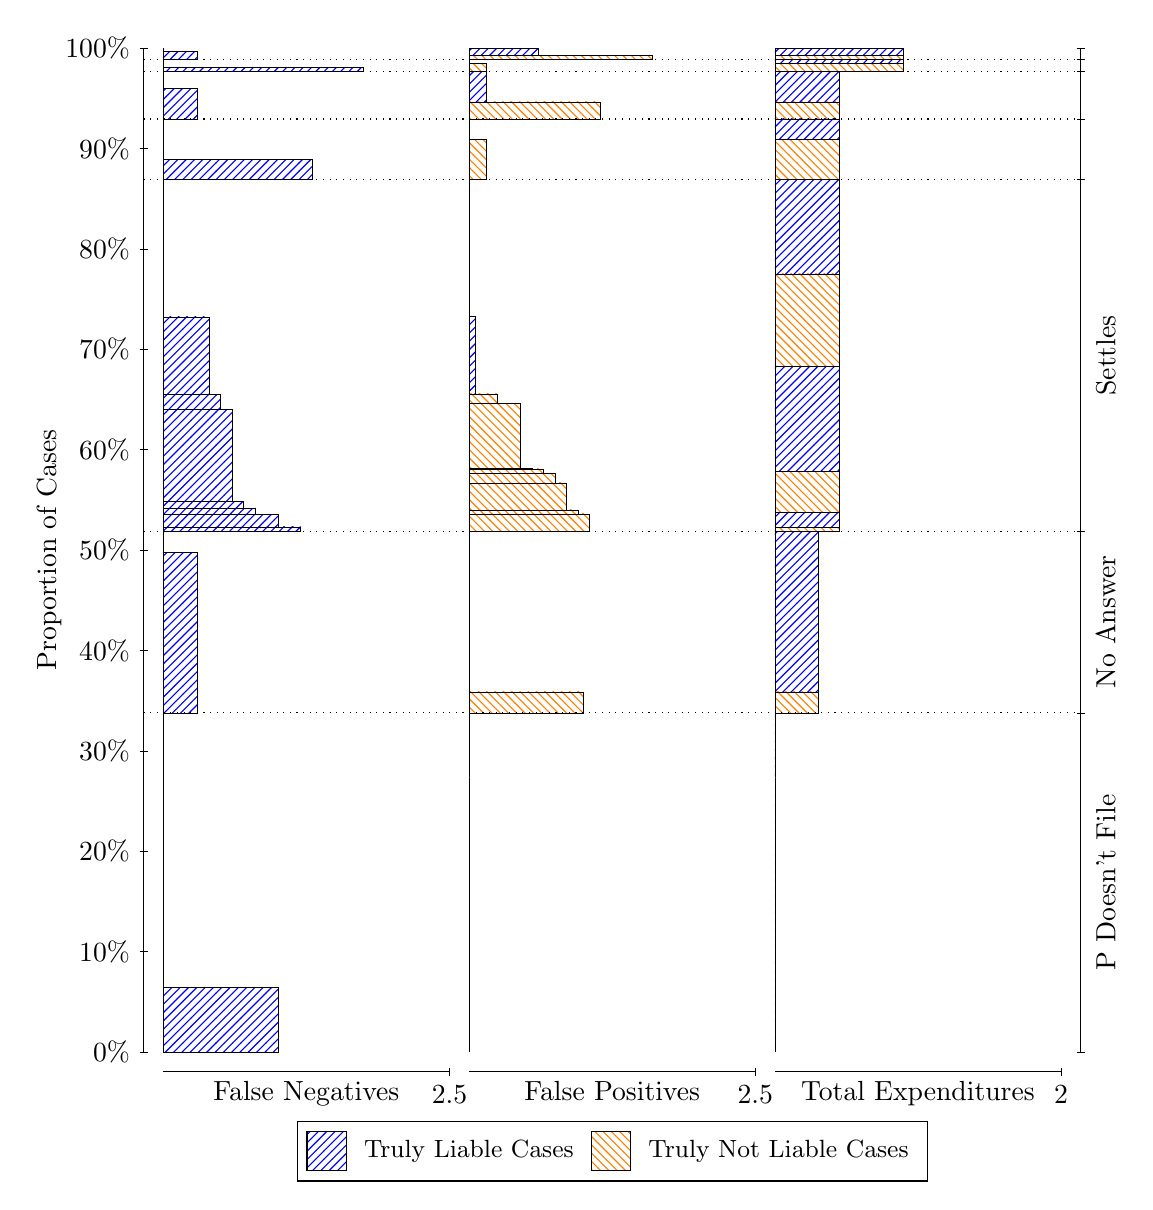
\begin{tikzpicture}
\draw[black, very thin] (1.5,1.75) -- (1.5,14.5);
\node[rotate=90, text=black, anchor=center] at (0.3, 8.125) {Proportion of Cases};
\draw[black, very thin] (1.45,1.75) -- (1.55,1.75);
\node[text=black, anchor=east] at (1.45, 1.75) {0\%};
\draw[black, very thin] (1.45,3.025) -- (1.55,3.025);
\node[text=black, anchor=east] at (1.45, 3.025) {10\%};
\draw[black, very thin] (1.45,4.3) -- (1.55,4.3);
\node[text=black, anchor=east] at (1.45, 4.3) {20\%};
\draw[black, very thin] (1.45,5.575) -- (1.55,5.575);
\node[text=black, anchor=east] at (1.45, 5.575) {30\%};
\draw[black, very thin] (1.45,6.85) -- (1.55,6.85);
\node[text=black, anchor=east] at (1.45, 6.85) {40\%};
\draw[black, very thin] (1.45,8.125) -- (1.55,8.125);
\node[text=black, anchor=east] at (1.45, 8.125) {50\%};
\draw[black, very thin] (1.45,9.4) -- (1.55,9.4);
\node[text=black, anchor=east] at (1.45, 9.4) {60\%};
\draw[black, very thin] (1.45,10.675) -- (1.55,10.675);
\node[text=black, anchor=east] at (1.45, 10.675) {70\%};
\draw[black, very thin] (1.45,11.95) -- (1.55,11.95);
\node[text=black, anchor=east] at (1.45, 11.95) {80\%};
\draw[black, very thin] (1.45,13.225) -- (1.55,13.225);
\node[text=black, anchor=east] at (1.45, 13.225) {90\%};
\draw[black, very thin] (1.45,14.5) -- (1.55,14.5);
\node[text=black, anchor=east] at (1.45, 14.5) {100\%};

\draw[black, very thin] (13.4,1.75) -- (13.4,14.5);
\draw[black, very thin] (13.35,1.75) -- (13.45,1.75);
\node[anchor=west] at (13.35, 1.75) {};
\draw[black, very thin] (13.35,6.0578) -- (13.45,6.0578);
\node[anchor=west] at (13.35, 6.0578) {};
\draw[black, very thin] (13.35,8.3627) -- (13.45,8.3627);
\node[anchor=west] at (13.35, 8.3627) {};
\draw[black, very thin] (13.35,12.83) -- (13.45,12.83);
\node[anchor=west] at (13.35, 12.83) {};
\draw[black, very thin] (13.35,13.599) -- (13.45,13.599);
\node[anchor=west] at (13.35, 13.599) {};
\draw[black, very thin] (13.35,14.205) -- (13.45,14.205);
\node[anchor=west] at (13.35, 14.205) {};
\draw[black, very thin] (13.35,14.356) -- (13.45,14.356);
\node[anchor=west] at (13.35, 14.356) {};
\draw[black, very thin] (13.35,14.5) -- (13.45,14.5);
\node[anchor=west] at (13.35, 14.5) {};

\draw[black, very thin, pattern color=blue, pattern=north east lines] (1.75,1.75) rectangle (3.2033,2.5713);
\draw[black, very thin, pattern color=orange, pattern=north west lines] (1.75,2.5713) rectangle (1.75,6.0578);
\draw[black, very thin, pattern color=blue, pattern=north east lines] (1.75,6.0578) rectangle (2.186,8.0987);
\draw[black, very thin, pattern color=orange, pattern=north west lines] (1.75,8.0987) rectangle (1.75,8.3627);
\draw[black, very thin, pattern color=blue, pattern=north east lines] (1.75,8.3627) rectangle (3.494,8.4181);
\draw[black, very thin, pattern color=blue, pattern=north east lines] (1.75,8.4181) rectangle (3.2033,8.5729);
\draw[black, very thin, pattern color=blue, pattern=north east lines] (1.75,8.5729) rectangle (3.058,8.5771);
\draw[black, very thin, pattern color=blue, pattern=north east lines] (1.75,8.5771) rectangle (2.9127,8.6517);
\draw[black, very thin, pattern color=blue, pattern=north east lines] (1.75,8.6517) rectangle (2.7673,8.7448);
\draw[black, very thin, pattern color=blue, pattern=north east lines] (1.75,8.7448) rectangle (2.622,9.9112);
\draw[black, very thin, pattern color=blue, pattern=north east lines] (1.75,9.9112) rectangle (2.4767,10.101);
\draw[black, very thin, pattern color=blue, pattern=north east lines] (1.75,10.101) rectangle (2.3313,11.085);
\draw[black, very thin, pattern color=orange, pattern=north west lines] (1.75,11.085) rectangle (1.75,12.83);
\draw[black, very thin, pattern color=blue, pattern=north east lines] (1.75,12.83) rectangle (3.6393,13.088);
\draw[black, very thin, pattern color=orange, pattern=north west lines] (1.75,13.088) rectangle (1.75,13.599);
\draw[black, very thin, pattern color=blue, pattern=north east lines] (1.75,13.599) rectangle (2.186,13.988);
\draw[black, very thin, pattern color=orange, pattern=north west lines] (1.75,13.988) rectangle (1.75,14.205);
\draw[black, very thin, pattern color=blue, pattern=north east lines] (1.75,14.205) rectangle (4.2933,14.252);
\draw[black, very thin, pattern color=orange, pattern=north west lines] (1.75,14.252) rectangle (1.75,14.356);
\draw[black, very thin, pattern color=blue, pattern=north east lines] (1.75,14.356) rectangle (2.186,14.453);
\draw[black, very thin, pattern color=orange, pattern=north west lines] (1.75,14.453) rectangle (1.75,14.5);
\draw[black, very thin, pattern color=orange, pattern=north west lines] (5.6333,1.75) rectangle (5.6333,5.2365);
\draw[black, very thin, pattern color=blue, pattern=north east lines] (5.6333,5.2365) rectangle (5.6333,6.0578);
\draw[black, very thin, pattern color=orange, pattern=north west lines] (5.6333,6.0578) rectangle (7.0867,6.3218);
\draw[black, very thin, pattern color=blue, pattern=north east lines] (5.6333,6.3218) rectangle (5.6333,8.3627);
\draw[black, very thin, pattern color=orange, pattern=north west lines] (5.6333,8.3627) rectangle (7.1593,8.585);
\draw[black, very thin, pattern color=orange, pattern=north west lines] (5.6333,8.585) rectangle (7.014,8.6333);
\draw[black, very thin, pattern color=orange, pattern=north west lines] (5.6333,8.6333) rectangle (6.8687,8.9776);
\draw[black, very thin, pattern color=orange, pattern=north west lines] (5.6333,8.9776) rectangle (6.7233,9.0931);
\draw[black, very thin, pattern color=orange, pattern=north west lines] (5.6333,9.0931) rectangle (6.578,9.1555);
\draw[black, very thin, pattern color=orange, pattern=north west lines] (5.6333,9.1555) rectangle (6.4327,9.1598);
\draw[black, very thin, pattern color=orange, pattern=north west lines] (5.6333,9.1598) rectangle (6.2873,9.9839);
\draw[black, very thin, pattern color=orange, pattern=north west lines] (5.6333,9.9839) rectangle (5.9967,10.108);
\draw[black, very thin, pattern color=blue, pattern=north east lines] (5.6333,10.108) rectangle (5.706,11.092);
\draw[black, very thin, pattern color=blue, pattern=north east lines] (5.6333,11.092) rectangle (5.6333,12.83);
\draw[black, very thin, pattern color=orange, pattern=north west lines] (5.6333,12.83) rectangle (5.8513,13.342);
\draw[black, very thin, pattern color=blue, pattern=north east lines] (5.6333,13.342) rectangle (5.6333,13.599);
\draw[black, very thin, pattern color=orange, pattern=north west lines] (5.6333,13.599) rectangle (7.3047,13.816);
\draw[black, very thin, pattern color=blue, pattern=north east lines] (5.6333,13.816) rectangle (5.8513,14.205);
\draw[black, very thin, pattern color=orange, pattern=north west lines] (5.6333,14.205) rectangle (5.8513,14.309);
\draw[black, very thin, pattern color=blue, pattern=north east lines] (5.6333,14.309) rectangle (5.6333,14.356);
\draw[black, very thin, pattern color=orange, pattern=north west lines] (5.6333,14.356) rectangle (7.9587,14.404);
\draw[black, very thin, pattern color=blue, pattern=north east lines] (5.6333,14.404) rectangle (6.5053,14.5);
\draw[black, very thin, pattern color=orange, pattern=north west lines] (9.5167,1.75) rectangle (9.5167,5.2365);
\draw[black, very thin, pattern color=blue, pattern=north east lines] (9.5167,5.2365) rectangle (9.5167,6.0578);
\draw[black, very thin, pattern color=orange, pattern=north west lines] (9.5167,6.0578) rectangle (10.062,6.3218);
\draw[black, very thin, pattern color=blue, pattern=north east lines] (9.5167,6.3218) rectangle (10.062,8.3627);
\draw[black, very thin, pattern color=orange, pattern=north west lines] (9.5167,8.3627) rectangle (10.334,8.4109);
\draw[black, very thin, pattern color=blue, pattern=north east lines] (9.5167,8.4109) rectangle (10.334,8.6007);
\draw[black, very thin, pattern color=orange, pattern=north west lines] (9.5167,8.6007) rectangle (10.334,9.1229);
\draw[black, very thin, pattern color=blue, pattern=north east lines] (9.5167,9.1229) rectangle (10.334,10.457);
\draw[black, very thin, pattern color=orange, pattern=north west lines] (9.5167,10.457) rectangle (10.334,11.632);
\draw[black, very thin, pattern color=blue, pattern=north east lines] (9.5167,11.632) rectangle (10.334,12.83);
\draw[black, very thin, pattern color=orange, pattern=north west lines] (9.5167,12.83) rectangle (10.334,13.342);
\draw[black, very thin, pattern color=blue, pattern=north east lines] (9.5167,13.342) rectangle (10.334,13.599);
\draw[black, very thin, pattern color=orange, pattern=north west lines] (9.5167,13.599) rectangle (10.334,13.816);
\draw[black, very thin, pattern color=blue, pattern=north east lines] (9.5167,13.816) rectangle (10.334,14.205);
\draw[black, very thin, pattern color=orange, pattern=north west lines] (9.5167,14.205) rectangle (11.152,14.309);
\draw[black, very thin, pattern color=blue, pattern=north east lines] (9.5167,14.309) rectangle (11.152,14.356);
\draw[black, very thin, pattern color=orange, pattern=north west lines] (9.5167,14.356) rectangle (11.152,14.404);
\draw[black, very thin, pattern color=blue, pattern=north east lines] (9.5167,14.404) rectangle (11.152,14.5);
\draw[black, dotted] (1.5,6.0578) -- (13.4,6.0578);
\draw[black, dotted] (1.5,8.3627) -- (13.4,8.3627);
\draw[black, dotted] (1.5,12.83) -- (13.4,12.83);
\draw[black, dotted] (1.5,13.599) -- (13.4,13.599);
\draw[black, dotted] (1.5,14.205) -- (13.4,14.205);
\draw[black, dotted] (1.5,14.356) -- (13.4,14.356);
\draw[black, very thin] (1.75,1.5) -- (5.3833,1.5);
\node[text=black, anchor=north] at (3.5667, 1.5) {False Negatives};
\draw[black, very thin] (5.3833,1.45) -- (5.3833,1.55);
\node[text=black, anchor=north] at (5.3833, 1.45) {2.5};

\draw[black, very thin] (5.6333,1.5) -- (9.2667,1.5);
\node[text=black, anchor=north] at (7.45, 1.5) {False Positives};
\draw[black, very thin] (9.2667,1.45) -- (9.2667,1.55);
\node[text=black, anchor=north] at (9.2667, 1.45) {2.5};

\draw[black, very thin] (9.5167,1.5) -- (13.15,1.5);
\node[text=black, anchor=north] at (11.333, 1.5) {Total Expenditures};
\draw[black, very thin] (13.15,1.45) -- (13.15,1.55);
\node[text=black, anchor=north] at (13.15, 1.45) {2};

\node[text=black, centered, rotate=90] at (13.72, 3.9039) {P Doesn't File};
\node[text=black, centered, rotate=90] at (13.72, 7.2102) {No Answer};
\node[text=black, centered, rotate=90] at (13.72, 10.596) {Settles};





\draw (7.449999999999999,1.5) node[draw=none] (baseCoordinate) {};
\begin{scope}[align=center]
        \matrix[scale=0.5, draw=black, below=0.5cm of baseCoordinate, nodes={draw}, column sep=0.1cm]{
            \node[rectangle, draw, minimum width=0.5cm, minimum height=0.5cm, pattern color=blue, pattern=north east lines] {}; &
            \node[draw=none, font=\small, text=black] (B) {Truly Liable Cases}; &
            \node[rectangle, draw, minimum width=0.5cm, minimum height=0.5cm, pattern color=orange, pattern=north west lines] {}; &
            \node[draw=none, font=\small, text=black] (B) {Truly Not Liable Cases}; \\
            };
\end{scope}

\end{tikzpicture}
\end{document}